\documentclass{article}
\usepackage[footnotes,definitionLists,hashEnumerators,smartEllipses,hybrid]{markdown}
\usepackage[utf8]{inputenc}
\usepackage[document]{ragged2e} % remove line justify

\usepackage{microtype}
\usepackage[none]{hyphenat}
 \usepackage{setspace}
	%\setstretch{1.2} %SOPHIA 
	
\usepackage{fontspec}
\defaultfontfeatures{Mapping=tex-text,Scale=MatchLowercase} %SOPHIA
\setmainfont{Source Sans Pro-Light
}[BoldFont={Source Sans Pro-Regular},
 ItalicFont={Source Sans Pro-Light Italic},
 ] %SOPHIA
 
\usepackage{xcolor}
\definecolor{sophiablue}{HTML}{0A2E4A}
\definecolor{sophiapink}{HTML}{E32A5C}
 \color{sophiablue} %SOPHIA
 
\usepackage{authblk} % authors

\usepackage{lineno} % used along with \linenumbers after begin document. 
\usepackage{setspace} % line spacing
  \setstretch{1.4}
\usepackage{enumitem}
\usepackage{microtype} % Creates better spaced text
\usepackage{siunitx} % SI units 

\usepackage{xcolor} % Setting colours and their usage
  \definecolor{natureblue}{RGB}{5,110,210}

\usepackage[colorlinks]{hyperref} % Colour for hyperlinks, (URLs, citations, cross reference)
  \AtBeginDocument{%this allows colours to change from the defined article template.
  \hypersetup{
  linkcolor={sophiapink},
  citecolor={sophiapink},
  filecolor=blue!50!black,
  urlcolor=sophiapink,
  }}

\usepackage{natbib}
  \setcitestyle{square,numbers,sort&compress}
  \setcitestyle{sort&compress}
\usepackage{hypernat} % hypernat also required to allow citations to compress. 
\usepackage{graphicx}
\graphicspath{ {images/} } % sets the path to image files (Figures)

\usepackage{booktabs} % required for tables
\usepackage{rotating,tabularx} % tabularx is the table style used, rotating can also be used
\newcolumntype{Z}{ >{\centering\arraybackslash}X } % defining table content layout per box
\usepackage{ltablex} % allow page break between lines in tabularx
\usepackage{caption} \captionsetup{font=normalsize} % to set the caption size as normal even when table is tiny.

\usepackage{pdflscape} % for rotated table
\usepackage{multirow} % for table

\begin{document}
\date{} %don't want date printed
%make title bold and 14 pt font (Latex default is non-bold, 16 pt)
\title{\Large \bf Comparison of two target sequencing approaches.
\footnote{This document's source code is available from the 
\href{https://github.com/DylanLawless/kit_assess}{GitHub repository}.
All code used in this report is available on the 
\href{https://github.com/DylanLawless/kit_assess}{GitHub repository}.}
}
%\thanks {Use thanks if u you need it}
%for single author (just remove % characters)

\author[1]{\rm Dylan Lawless, PHD}
\affil[1]{Global Health Institute, School of Life Sciences, École Polytechnique Fédérale de Lausanne, Switzerland, 
\color{sophiapink}{Dylan.Lawless@epfl.ch}
}
%\affil[ ]{\textit {\{email1,email2,email3,email4\}@xyz.edu}}
\maketitle
%\linenumbers

%\cite{•}

\section{Introduction}
\label{intro}
The two datasets (S1 and S2) of paired-end short reads are from the SAME human DNA NGS library for clinical diagnosis of solid tumor. 
They were obtained through two different target sequencing approaches with corresponding target region file provided (hg19). 
Herein, we evaluate their performances for use in clinical diagnose.

\section{Result summary}
Method evaluated using X performed better than Y for use in clinical diagnosis of solid tumor.
\begin{markdown}

\section{Main files for technical writing report}
\textit{Note:}
This section contains the main information required for a technical report.
The remainder of this document contains additional information which is \textit{not} required for further reports, and includes duplicate references to to files listed here.
Please include:

* \textbf{Introduction}: all details from sec. \ref{intro}.
* \textbf{Data source}: all details from sec. \ref{data_source}.
* \textbf{Protocol details}: a hyperlink to the protocol source: [\href{https://github.com/DylanLawless/kit_assess/README.md}{link}].
* \textbf{Main result}: Summary 
* \textbf{Figures}: list of figures




\section{Methods}
\subsection{Data source}
 \label{data_source}

* Description: The sequencing group performed library preparation for two (2) samples (AH and CH) using \href{https://www.sophiagenetics.com/clinical/oncology/solid-tumors/}{Kit X}.
The performance of each was assessed with several bioinformatic methods including read quality control and performance when aligning to reference genome
[\href{https://github.com/DylanLawless/kit_assess}{code available here}].
* Data source: raw sequence data was received from
 [\href{https://www.sophiagenetics.com}{link group and contact address}].
* Date: 2022-02-14
* Link to tickets where their submission was logged: [\href{https://www.sophiagenetics.com}{link}]
* Data integrity: [\href{https://github.com/DylanLawless/kit_assess/src/metadata/raw.md5sum}{link metadata md5sum}].



\subsection{Configuration}

* Local env: macOS v11.6 \href{https://support.apple.com/macos}{software}
* Remote env: Red Hat Enterprise Linux Server 7.6 (Maipo)  \href{https://www.redhat.com/en/technologies/linux-platforms/enterprise-linux}{software}
* compiler intel: (19.0.5 and 19.1.1)
\href{https://www.intel.com/content/www/us/en/developer/tools/oneapi/commercial-base-hpc.html#gs.ppyt3x}{software}
* R: R v4.1.0 Camp Pontanezen  \href{https://www.r-project.org}{software}
* R libraries: versions unlisted
* fastqc: v0.11.7 \href{https://www.bioinformatics.babraham.ac.uk/projects/fastqc/}{software}
* samtools: v1.10 \href{https://www.htslib.org}{software}
* bwa: v0.7.17 \href{https://janis.readthedocs.io/en/latest/tools/bioinformatics/bwa/bwamem.html}{software}
* picard: v2.20.8  \href{http://broadinstitute.github.io/picard/}{software}

\subsection{Data exploration}
* Read counts: 

read_count.sh
3. fastQC: manual run all fastq and save to ./processed/fastqc
3. fastqcr: Assess fastqc rerpots further
4. src/target_info.sh
5. src/1.trim.sh
6. src/2.align.sh
7. src/3.sort.sh
8. src/mapping.sh



\section{Supplemental files for intermediate report}
 [\href{https://github.com/DylanLawless/kit_assess/data/processed/}{link}].
 

\section{Result details}

\begin{figure}[ht] \hspace*{0cm} 
\begin{center}
    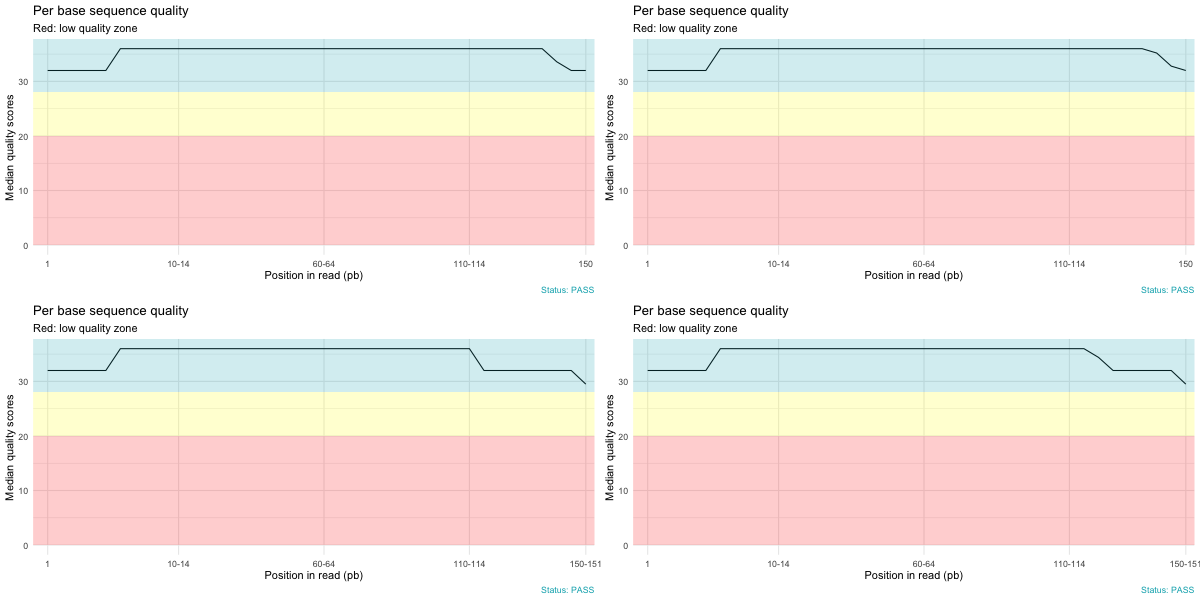
\includegraphics[scale=0.3]{p1}
    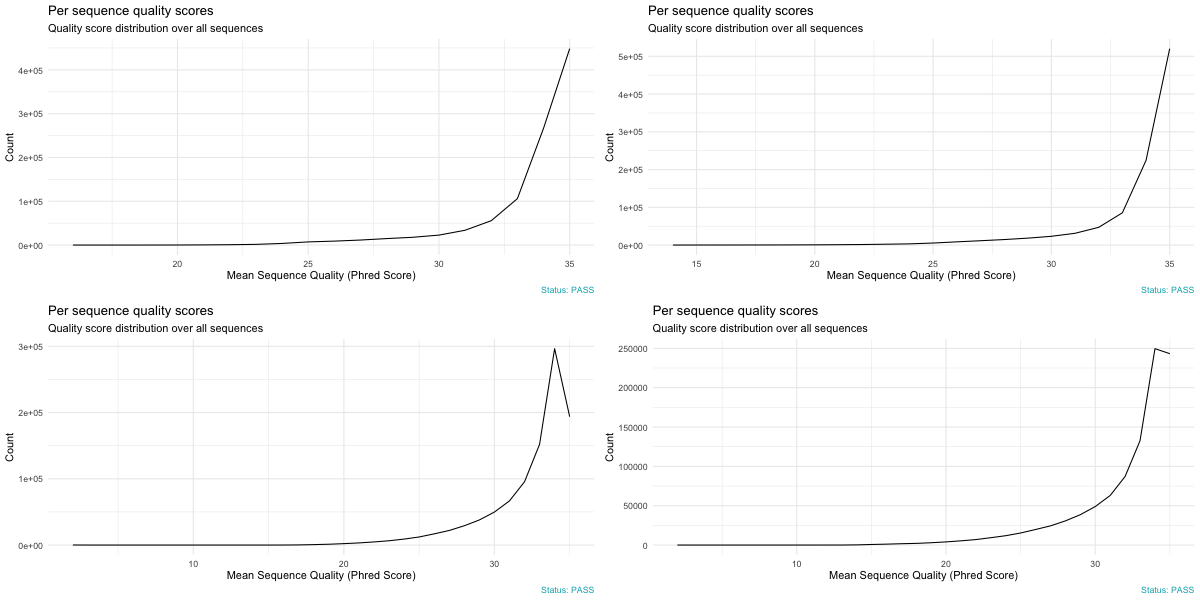
\includegraphics[scale=0.3]{p2}
	\caption{Caption.}
	\label{fig:p1p2}
\end{center}
\end{figure}

\begin{figure}[ht] \hspace*{0cm} 
\begin{center}
    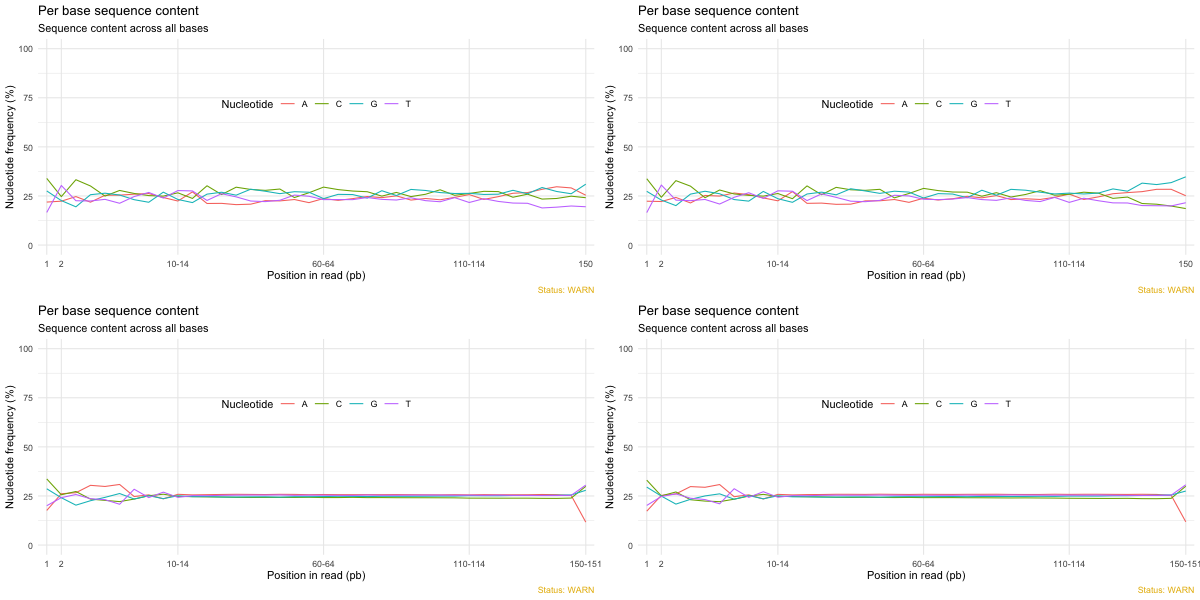
\includegraphics[scale=0.3]{p3}
    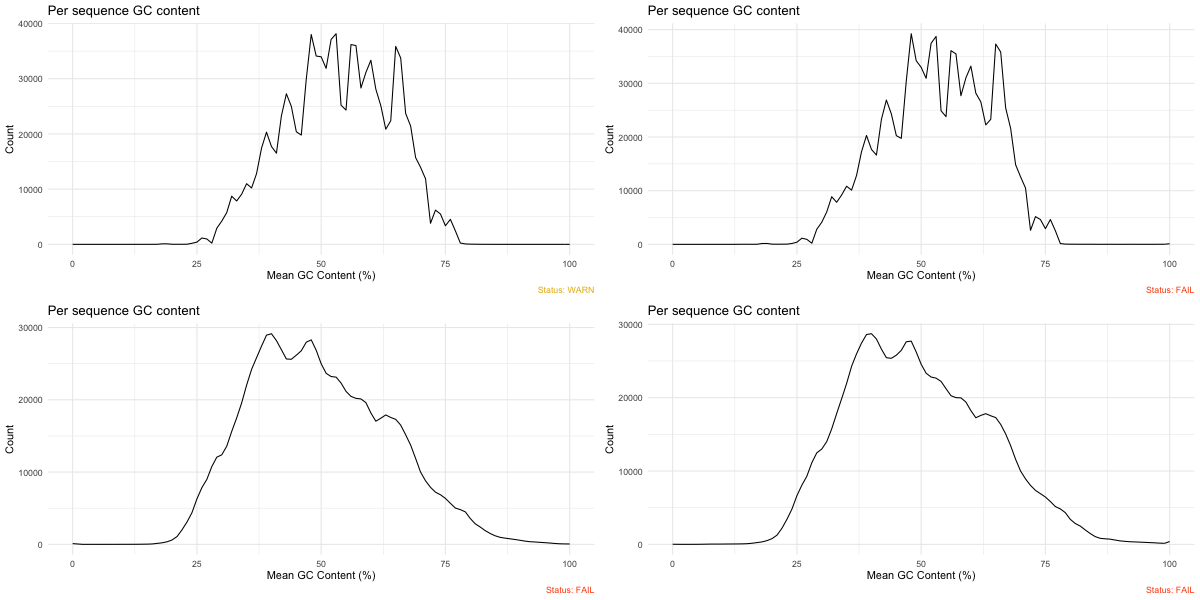
\includegraphics[scale=0.3]{p4}
	\caption{Caption.}
	\label{fig:p3p4}
\end{center}
\end{figure}

\begin{figure}[ht] \hspace*{0cm} 
\begin{center}
    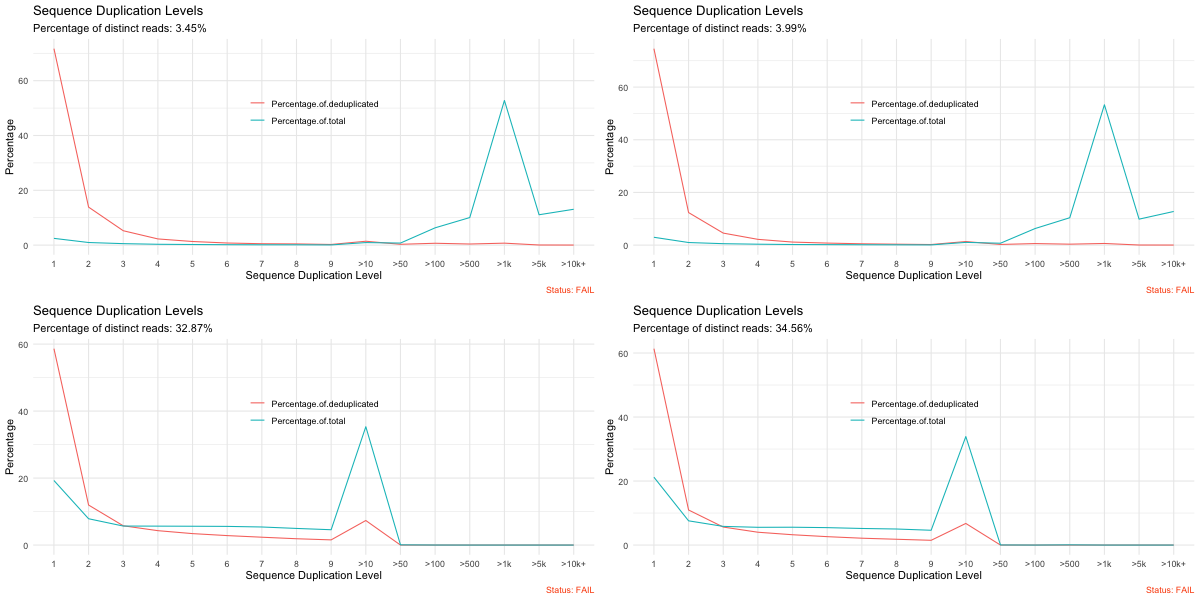
\includegraphics[scale=0.3]{p5}
    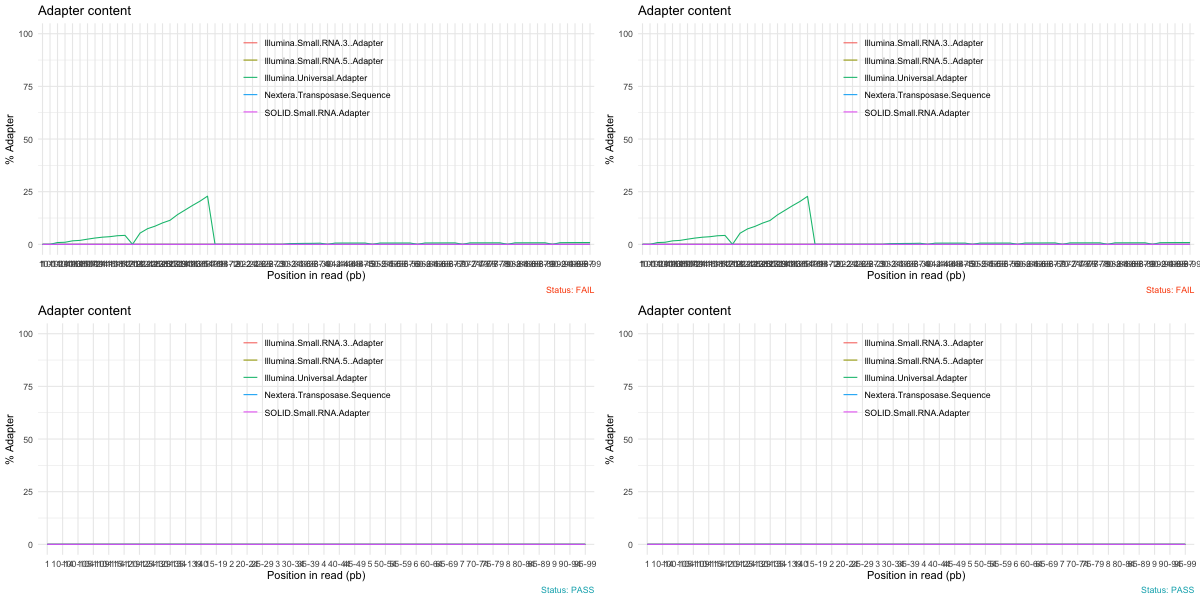
\includegraphics[scale=0.3]{p6}
	\caption{Caption.}
	\label{fig:p5p6}
\end{center}
\end{figure}


\section{Methods}

\end{markdown}
\bibliographystyle{unsrtnat}
\bibliography{references}

\end{document}


